\subsubsection{Infinite potential well}
What happens when $V_0 \to \infty$, in this case particle can't leave the well, i.e. $\psi(x)= 0$.
	
So we already have the solution:
$$\psi(x) = \begin{cases}
Ae^{\frac{ipx}{\hbar}} +Be^{\frac{-ipx}{\hbar}} & 0<x<L\\
0 \\ \text{otherwise}
\end{cases}$$
From $\psi(0)=0$ we acquire that
$$\psi(x) = C\sin(\frac{ipx}{\hbar})$$
Since $C\neq=0$ we get that $p$ can aquire only particular values such that
$$\frac{pL}{\hbar} = n\pi$$
$$p=\frac{n\hbar \pi}{2}$$
Thus, since
$$H = \frac{p^2}{2m}$$
$$E_n = \frac{n^2\hbar^2 \pi^2}{2mL^2}$$
and
$$\psi = C \sin(\frac{n \pi x}{L})$$

\subsubsection{General case}
If we have piecewise constant potenetial:

\begin{center}
	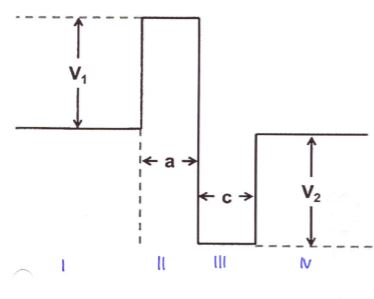
\includegraphics[width=0.4\linewidth]{./lect9/pic1.jpg}
\end{center}
For potential higher than energy we get decaying potential, and for each of wells we get oscillating solution.

\subsection{Bound states}
If we close to potential minimum, we can approximate it with Taylor series as
$$V \approx \frac{1}{2} m\omega^2 X^2$$
We will solve the Schr\"{o}dinger equation for harmonic oscillator:
$$H\ket{\psi_E} = E\ket{\psi_E}$$
For
$$H = \frac{p^2}{2m} + \frac{1}{2} m\omega^2 X^2$$
In position representation we get
$$-\frac{\hbar^2}{2m}\psi_E + \frac{1}{2}mw^2X^2\psi_E = E\psi_E$$
Lets perform variable substitution:
$$a = \sqrt{\frac{m\omega}{2\hbar}} X +i\frac{1}{\sqrt{2m\omega\hbar}} P$$
Since $X$, $P$ are Hermitian
$$a^\dagger = \sqrt{\frac{m\omega}{2\hbar}} X +i\frac{1}{\sqrt{2m\omega\hbar}} P$$
$$a^\dagger a = \frac{mw}{2\hbar}X^2 +\frac{P^2}{2m\omega\hbar } +\frac{1}{2\hbar} i(XP-PX) $$
$$a^\dagger a = \frac{mw}{2\hbar}X^2 +\frac{P^2}{2m\omega\hbar } +\frac{1}{2\hbar} i\comm{X}{P} $$
$$\comm{X}{P} = \hbar\comm{X}{K} = ih$$
Thus
$$H = \hbar \omega \qty(a^\dagger a + \frac{1}{2})$$

Denote $N=a^\dagger a$ and $N\ket{n} = n\ket{n}$. 

We can show that $n\geq 0$ and $$a\ket{n} =\begin{cases}
\ket{n-1}&n\neq0\\
0&n=0
\end{cases}$$
Which means than $n$ has to be integer.